\section{Case Study: 200 Nodes}
\subsection{Introduction}
In this chapter we want to analyze the case at 200 nodes, as it is the quantity that is halfway between our configurations. At the end of the simulations we decided to calculate the average coverage rate, summarized in this table.

\begin{table}[h!]
\centering
\begin{tabular}{|c|c|c|c|c|c|}
\hline
       & r=10    & r=30    & r=50    & r=75    & r=100   \\ \hline
p=0,15 & 0,90727 & 1       & 1       & 1       & 1       \\ \hline
p=0,3  & 0,89379 & 0,99924 & 0,99561 & 1       & 0,99924 \\ \hline
p=0,5  & 0,79909 & 0,99424 & 0,98803 & 0,98894 & 0,99591 \\ \hline
p=0,7  & 0,71045 & 0,97985 & 0,96455 & 0,93727 & 0,9903  \\ \hline
p=0,85 & 0,57303 & 0,94212 & 0,90212 & 0,91833 & 0,9797  \\ \hline
p=1    & 0,47545 & 0,81909 & 0,67121 & 0,76303 & 0,96727 \\ \hline
\end{tabular}
\caption{Mean coverage percentage}
\label{tab:my-table}
\end{table}

Since the mean didn't give enough information about the index variation, we decided to calculate the standard deviation as well.
\begin{table}[h!]
\centering
\begin{tabular}{|l|l|l|l|l|l|}
\hline
       & r=10    & r=30    & r=50    & r=75    & r=100   \\ \hline
p=0,15 & 0,16006 & 0       & 0       & 0       & 0       \\ \hline
p=0,3  & 0,12149 & 0,00283 & 0,01886 & 0       & 0,00435 \\ \hline
p=0,5  & 0,21101 & 0,00686 & 0,0454  & 0,02858 & 0,01618 \\ \hline
p=0,7  & 0,24243 & 0,02438 & 0,06648 & 0,09235 & 0,02274 \\ \hline
p=0,85 & 0,26813 & 0,06087 & 0,11409 & 0,11198 & 0,03477 \\ \hline
p=1    & 0,27804 & 0,14129 & 0,17092 & 0,12449 & 0,03833 \\ \hline
\end{tabular}
\caption{Standard deviation of the coverage percentage}
\label{tab:my-table}
\end{table}

In this way we have excluded the configurations with a difference between mean and standard deviation of the coverage rate less than 90\%. We are interested in configurations that have a satisfactory coverage percentage, as these situations model a reliable real system.
\begin{table}[h!]
\centering
\begin{tabular}{|l|l|l|l|l|l|}
\hline
       & r=10    & r=30                            & r=50                            & r=75                            & r=100                           \\ \hline
p=0,15 & 0,74721 & \cellcolor[HTML]{92D050}1       & \cellcolor[HTML]{92D050}1       & \cellcolor[HTML]{92D050}1       & \cellcolor[HTML]{92D050}1       \\ \hline
p=0,3  & 0,7723  & \cellcolor[HTML]{92D050}0,99641 & \cellcolor[HTML]{92D050}0,97674 & \cellcolor[HTML]{92D050}1       & \cellcolor[HTML]{92D050}0,99489 \\ \hline
p=0,5  & 0,58808 & \cellcolor[HTML]{92D050}0,98738 & \cellcolor[HTML]{92D050}0,94263 & \cellcolor[HTML]{92D050}0,96036 & \cellcolor[HTML]{92D050}0,97973 \\ \hline
p=0,7  & 0,46802 & \cellcolor[HTML]{92D050}0,95547 & 0,89807                         & 0,84492                         & \cellcolor[HTML]{92D050}0,96756 \\ \hline
p=0,85 & 0,3049  & 0,88125                         & 0,78803                         & 0,80636                         & \cellcolor[HTML]{92D050}0,94492 \\ \hline
p=1    & 0,19741 & 0,67781                         & 0,5003                          & 0,63854                         & \cellcolor[HTML]{92D050}0,92895 \\ \hline
\end{tabular}
\caption{Run that we decide to analyze}
\label{tab:my-table}
\end{table}

\section{Performance indexes}
After selecting the runs to be analysed, we chose to plot the most interesting performance indicators such as the percentage of collisions, coverage and the completion time of each scenario. For symmetry, the graphs also show configurations, such as the one with probability 0.7 and radius 75, which we had previously rejected.

\subsection{Coverage percentage}
\begin{figure}[h!]
\centering
    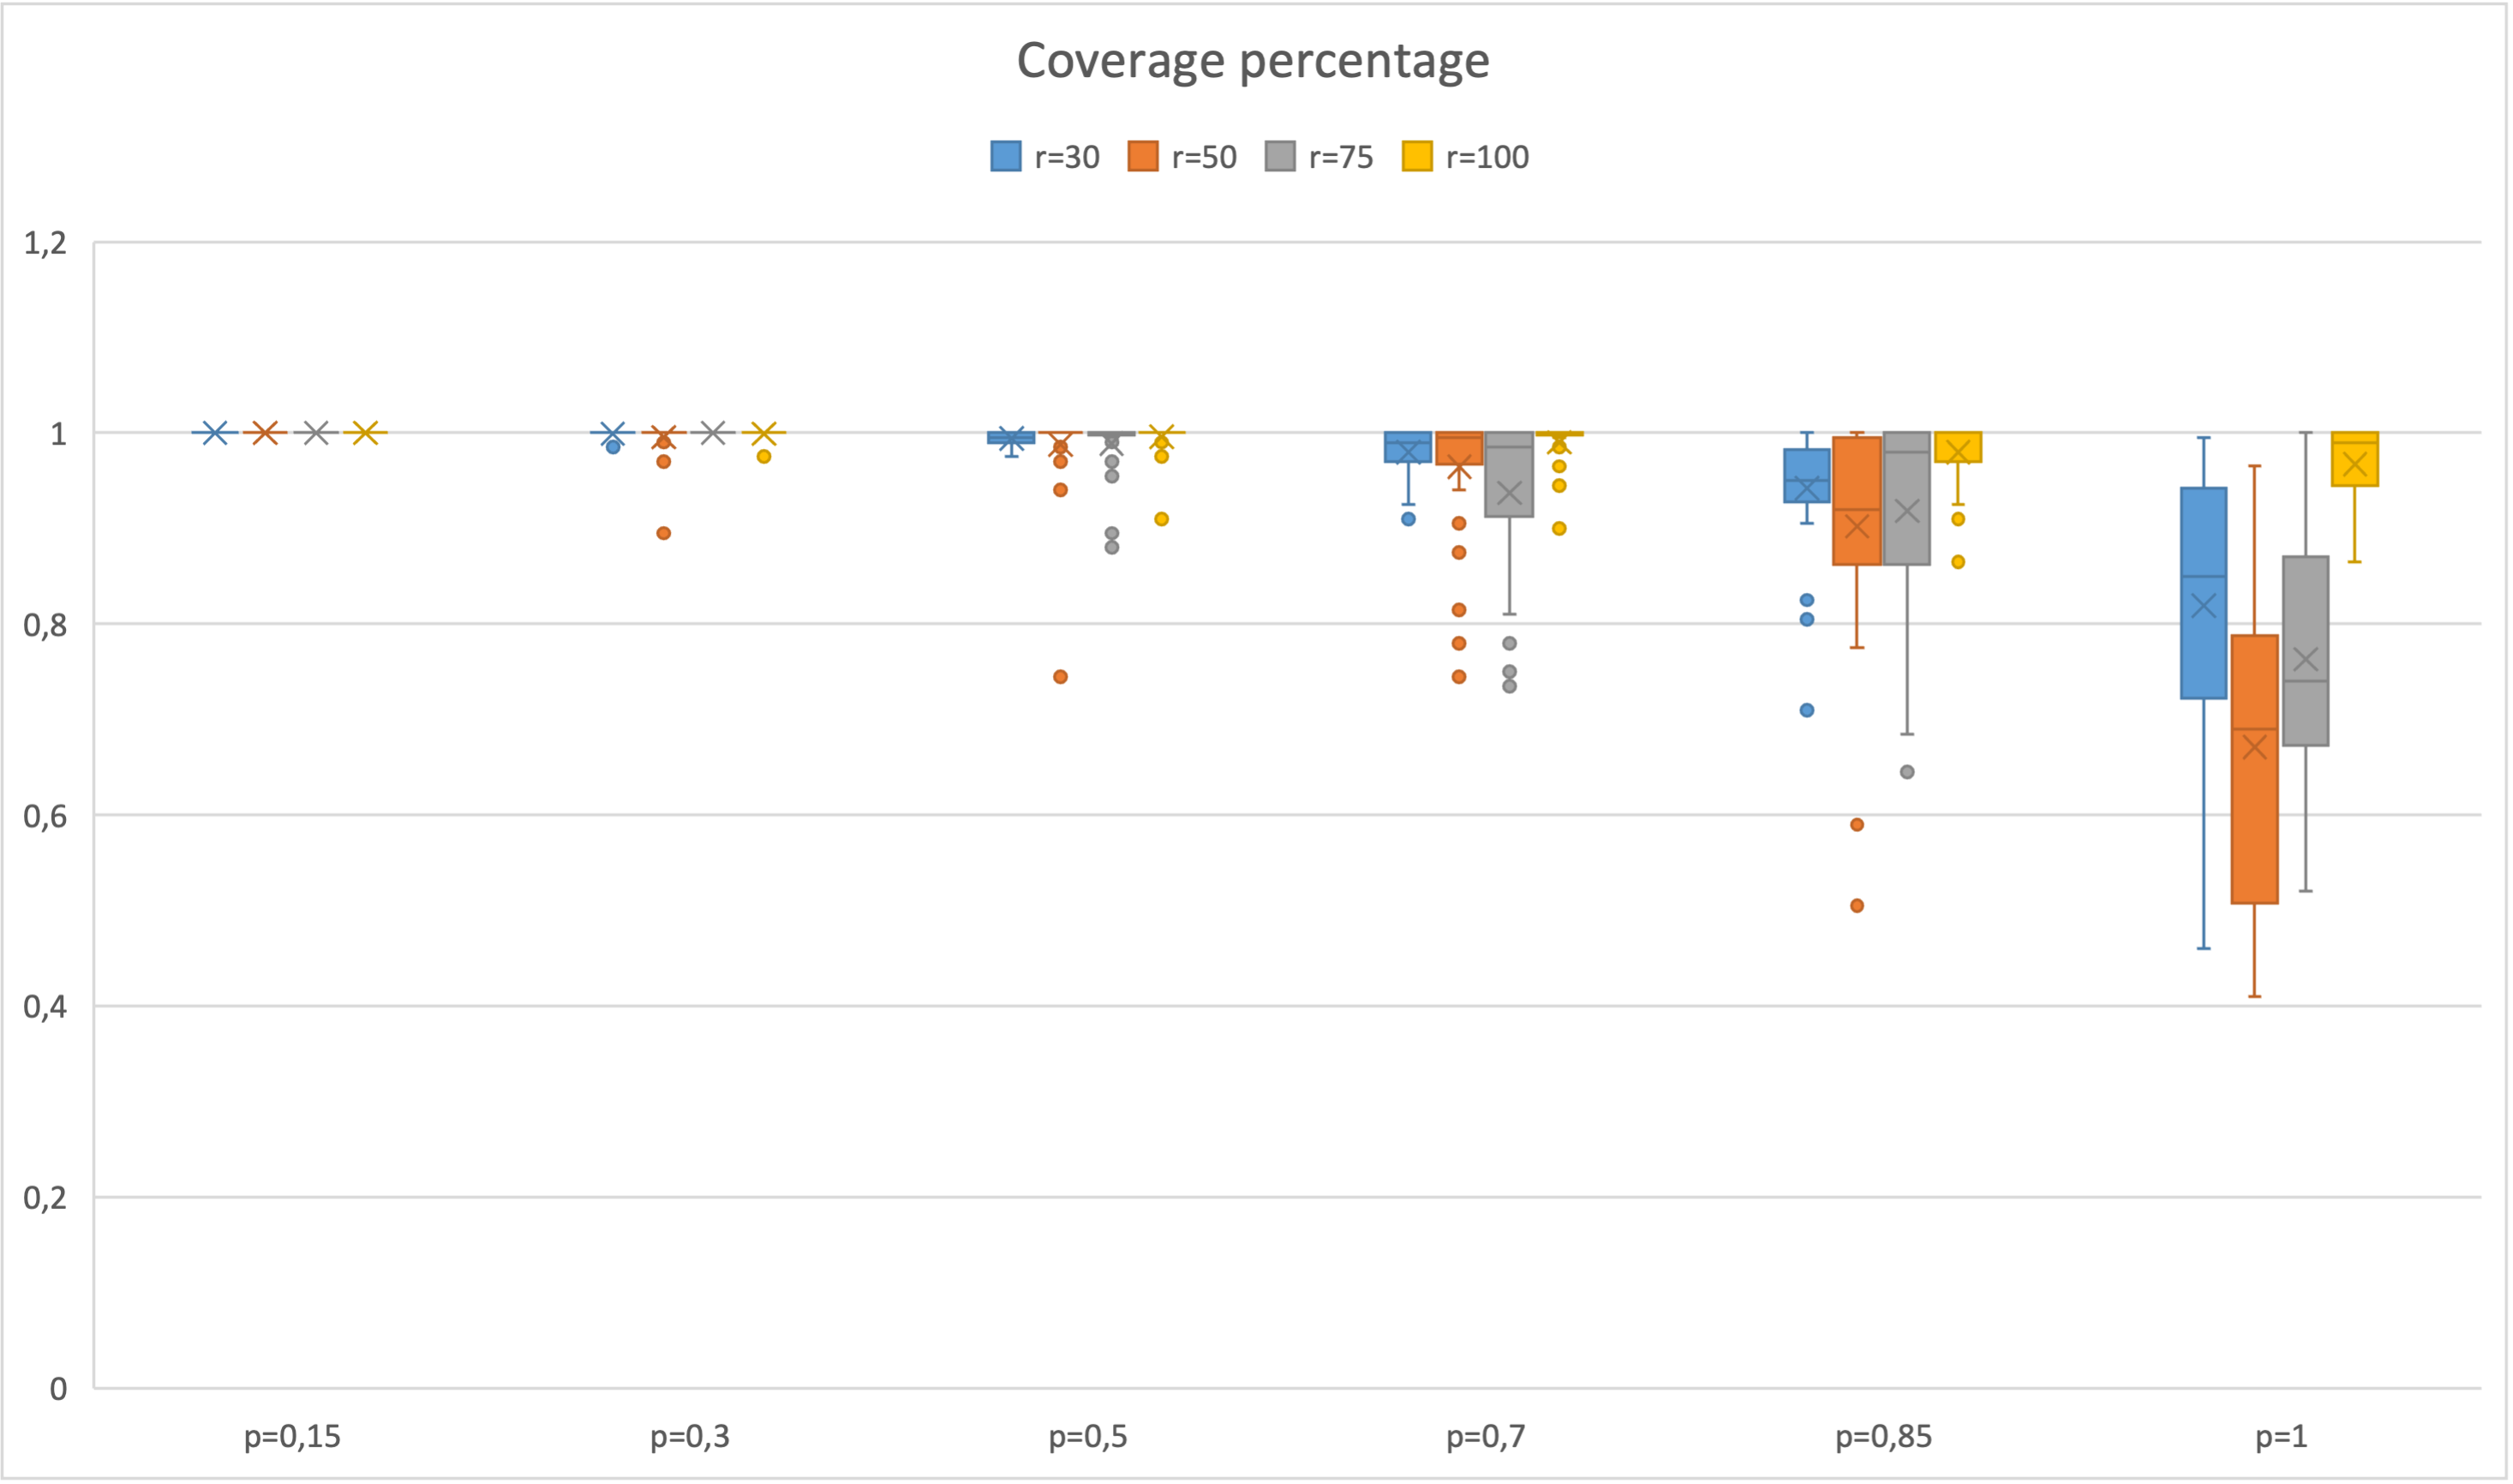
\includegraphics[width= 1\textwidth]{./images/Rate200Boxplot.png}
    \caption{Coverage percentage}
    \label{fig:immagine}
\end{figure}

\noindent Looking at this graph, it can be seen that increasing the probability does not give better coverage in most cases, as one would expect. In fact, it should be emphasized that as the probability increases, collisions also increase accordingly.

\subsection{Coverage time}
\begin{figure}
\centering
    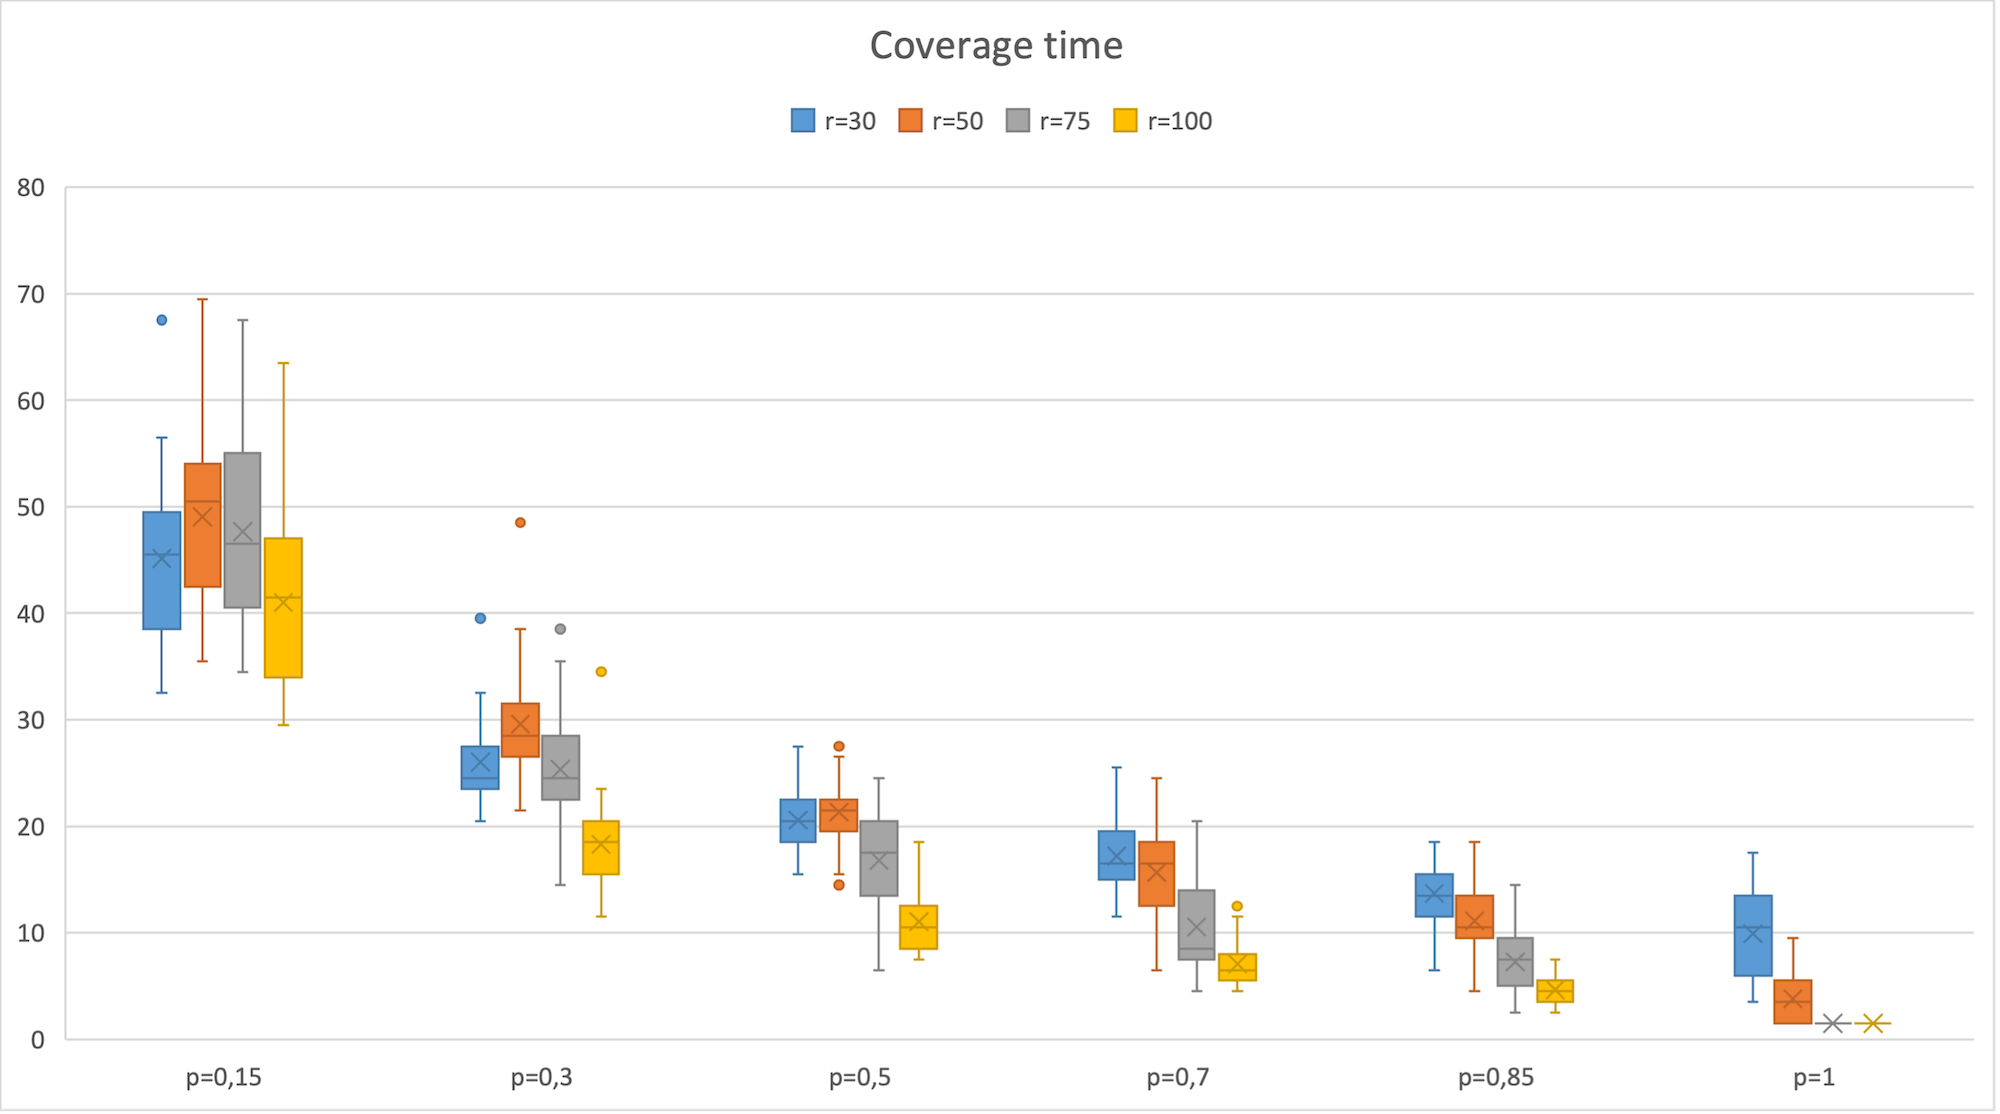
\includegraphics[width= 1\textwidth]{./images/Time200Boxplot.png}
    \caption{Coverage time}
    \label{fig:immagine}
\end{figure}
\noindent As imagined, the coverage time decreases as the probability increases, as a higher probability translates into more nodes that can send the infection message.

\subsection{Mean collision rate}

\begin{figure}
\centering
    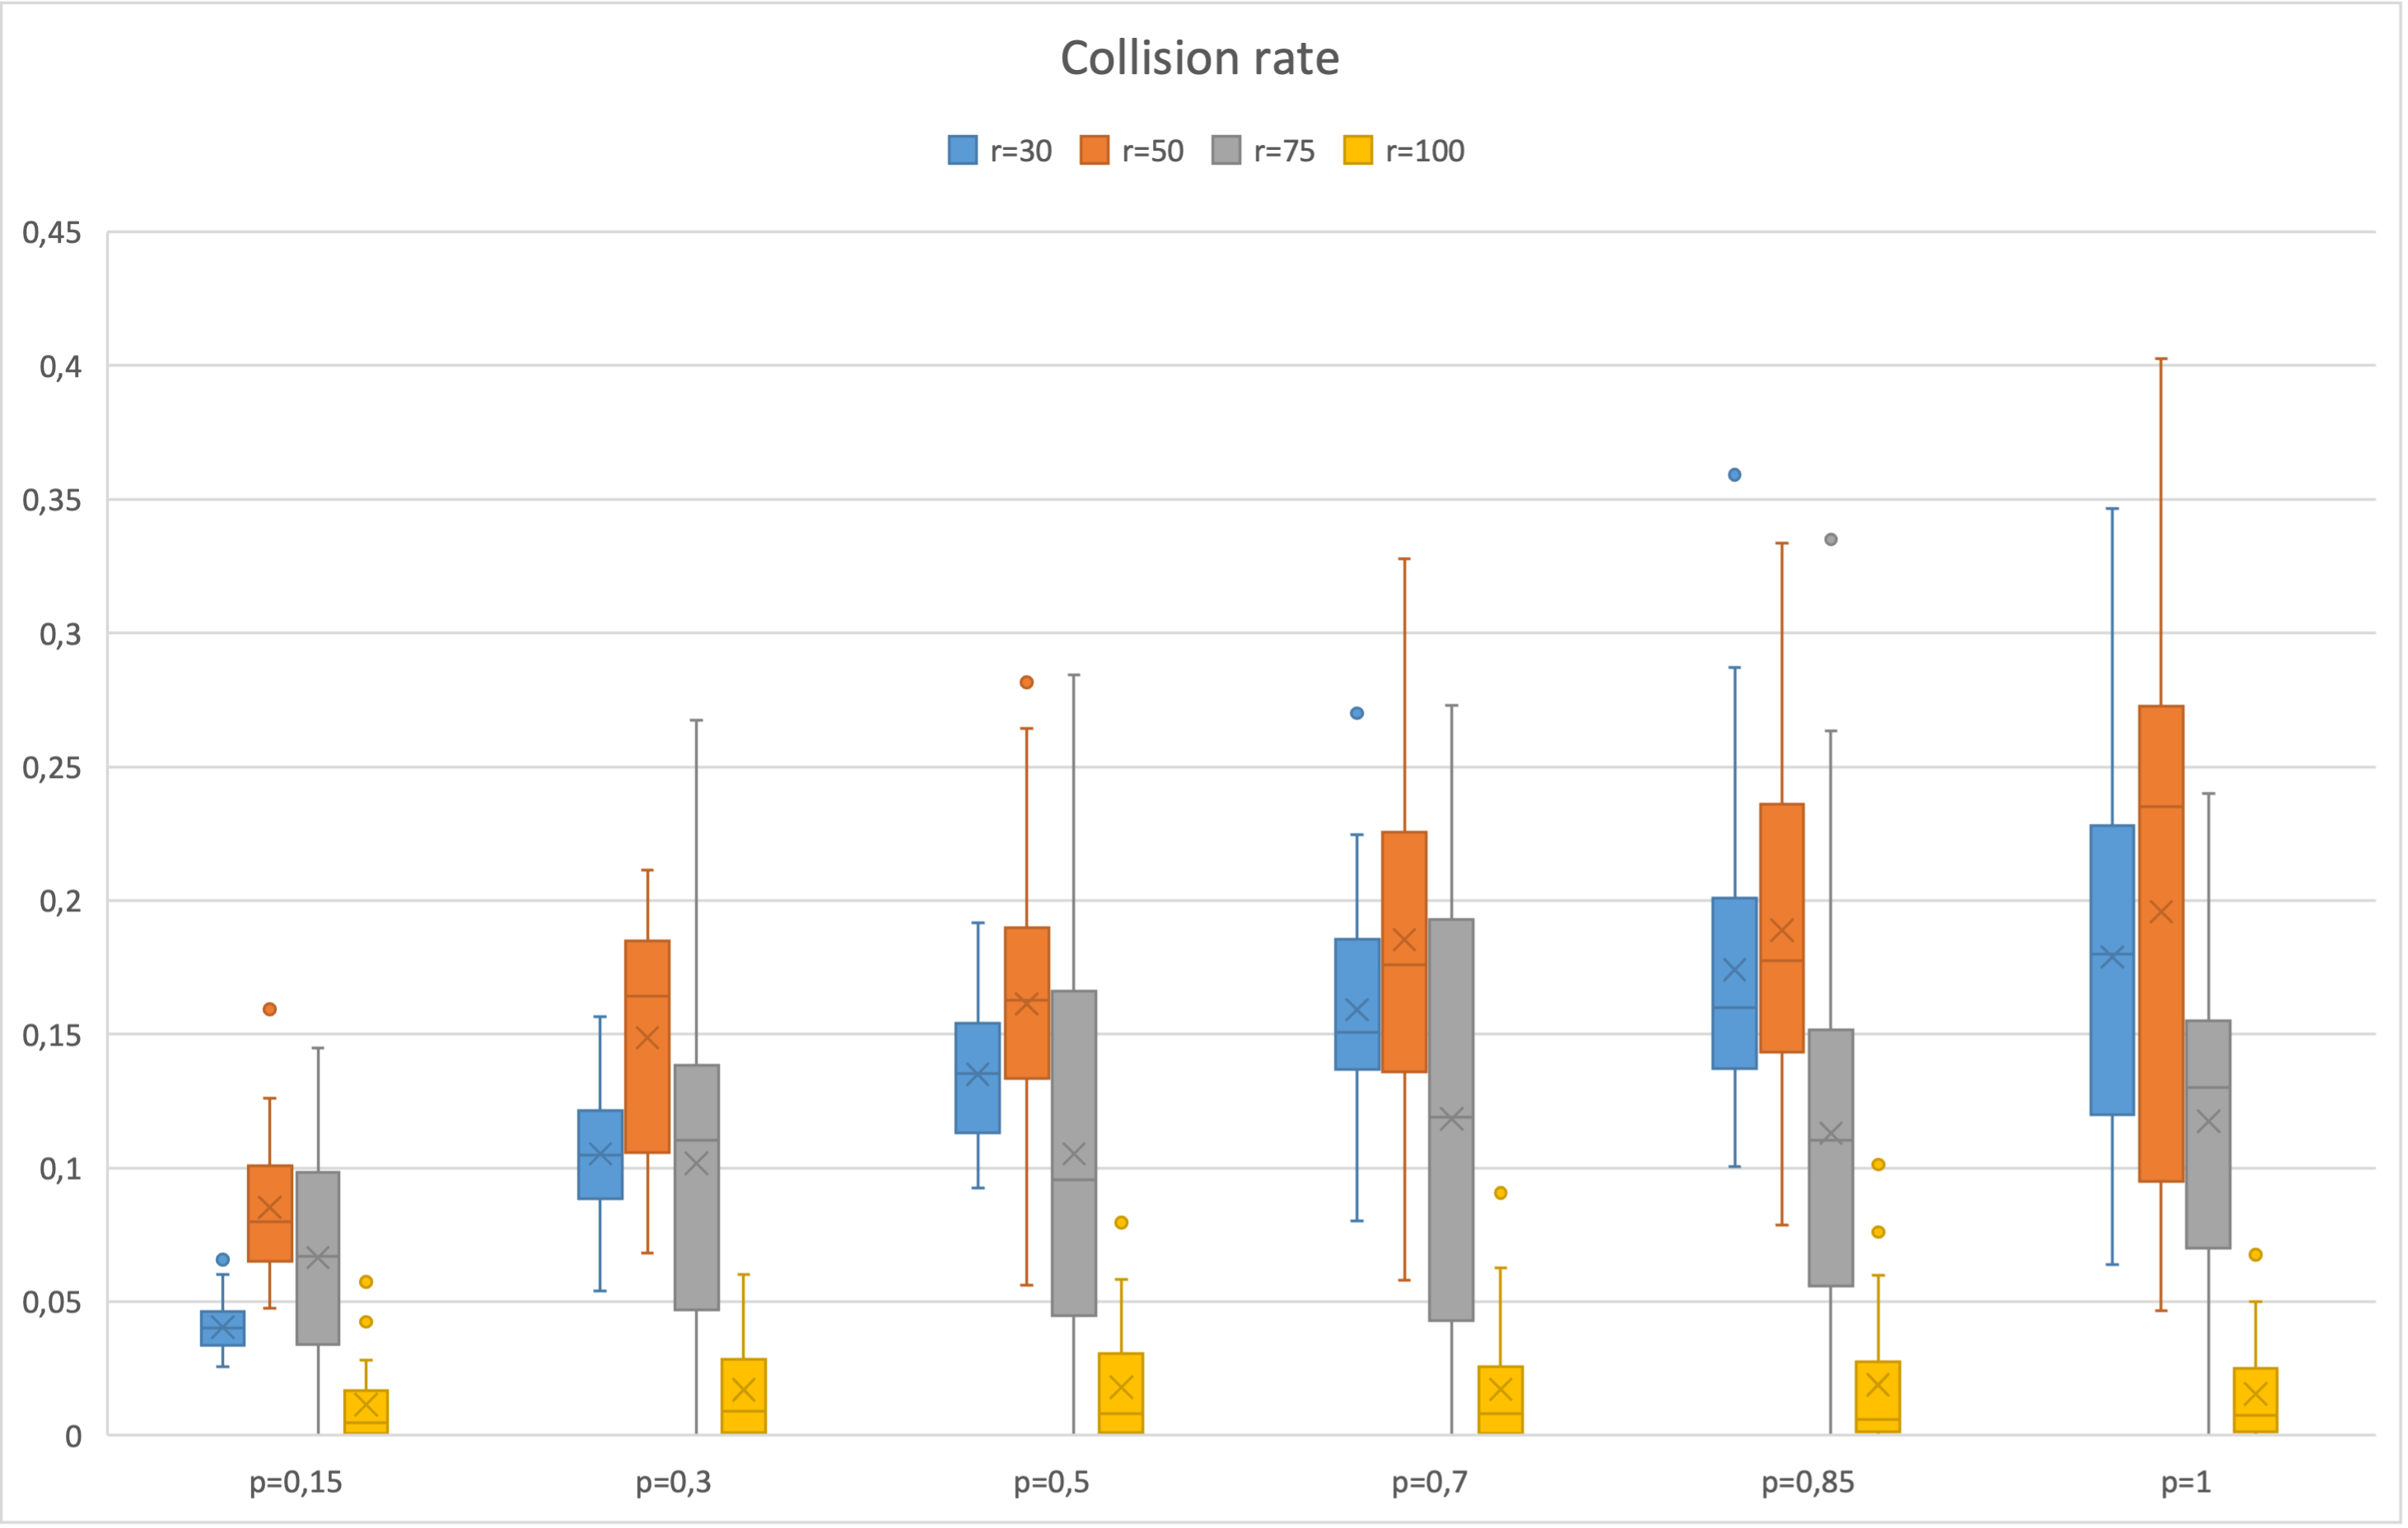
\includegraphics[width= 1\textwidth]{./images/Collision200Boxplot.png}
    \caption{Mean collision rate}
    \label{fig:immagine}
\end{figure}

\noindent As regards the collision index, the average value from the initial instant to the completion instant was obtained for all 33 runs. It was not possible to detect clearly visible trends, as for radius 30 and 50 collisions increase on average as the probability increases, while a decrease is noted for 75 and a more or less stationary situation for radius 100
